
\setlength{\tabcolsep}{2pt}
\renewcommand{\arraystretch}{0.8}
\begin{figure*}[h!]
	\tiny
	\centering 	\tiny
	\begin{tabular}{l|rrr|rrr|rrr||rrr|rrr|rrr||rrr|rrr|rrr}
		& \multicolumn{9}{c||}{0.25} & \multicolumn{9}{c||}{0.5} & \multicolumn{9}{c}{0.75}\\
		& \multicolumn{3}{c|}{coverage} & \multicolumn{3}{c|}{avg time} & & & & \multicolumn{3}{c|}{covergae} & \multicolumn{3}{c|}{avg time} & & & & \multicolumn{3}{c|}{coverage} & \multicolumn{3}{c|}{avg time} & & &\\\hline
		& C & C nr & max & C & C nr & max & \#gs & \#n & fn & C & C nr & max & C & C nr & max & \#gs & \#n & fn & C & C nr & max & C & C nr & max & \#gs & \#n & fn\\\hline
		airport (28) & 0.93 & 0.93 & 0.86 & 0.0179 & 0.0296 & 15.5606 & 2.4 & 8.7 & 0.76 & 0.71 & 0.75 & 0.68 & 8.1089 & 3.8531 & 2.5639 & 1.9 & 4.4 & 0.71 & 0.57 & 0.57 & 0.68 & 3.4586 & 2.4734 & 0.256 & 1.0 & 2.4 & 0.61\\
		barman (4) & 1.00 & 1.00 & 1.00 & 0.003 & 0.0075 & 0.0382 & 3.0 & 7.0 & 0.88 & 1.00 & 1.00 & 1.00 & 42.121 & 26.4318 & 4.7071 & 3.0 & 7.0 & 0.88 & 0.00 & 0.00 & 1.00 & - & - & - & - & - & -\\
		blocks (28) & 1.00 & 0.93 & 0.96 & 0.0003 & 0.0006 & 0.0045 & 6.2 & 391.6 & 0.96 & 0.96 & 0.93 & 0.75 & 0.0006 & 0.0022 & 0.2815 & 6.6 & 138.7 & 0.93 & 0.89 & 0.86 & 0.61 & 0.0037 & 0.0072 & 0.7265 & 6.1 & 50.9 & 0.72\\
		data-net (12) & 0.00 & 0.00 & 1.00 & - & - & - & - & - & - & 0.00 & 0.00 & 1.00 & - & - & - & - & - & - & 0.00 & 0.00 & 1.00 & - & - & - & - & - & -\\
		depot (7) & 1.00 & 1.00 & 1.00 & 0.001 & 0.0027 & 0.065 & 4.0 & 36.1 & 0.94 & 1.00 & 1.00 & 1.00 & 1.2503 & 0.325 & 5.7004 & 7.0 & 34.6 & 0.91 & 0.43 & 0.43 & 0.57 & 4.9737 & 0.767 & 3.0968 & 2.7 & 11.0 & 0.68\\
		driverlog (13) & 1.00 & 1.00 & 1.00 & 0.0002 & 0.0007 & 0.0221 & 7.0 & 553.9 & 0.98 & 0.85 & 0.92 & 0.77 & 0.0062 & 0.0167 & 0.1872 & 13.4 & 387.4 & 0.86 & 0.69 & 0.69 & 0.62 & 2.4397 & 0.8843 & 4.7626 & 7.9 & 189.8 & 0.49\\
		elevators (40) & 0.00 & 0.00 & 1.00 &  &  &  &  &  &  & 0.00 & 0.00 & 1.00 & - & - & - & - & - & - & 0.00 & 0.00 & 0.83 & - & - & - & - & - & -\\
		floortile (13) & 0.54 & 0.46 & 0.46 & 0.0027 & 0.0077 & 0.0846 & 88.7 & 2881.7 & 0.99 & 0.15 & 0.15 & 0.15 & 0.4098 & 0.0973 & 0.3864 & 66.0 & 407.5 & 0.80 & 0.08 & 0.15 & 0.15 & 10.6455 & 2.4284 & 1.6908 & 30.0 & 142.0 & 0.28\\
		freecell (15) & 1.00 & 1.00 & 1.00 & 0.0007 & 0.004 & 0.1086 & 4.0 & 15.0 & 0.94 & 1.00 & 1.00 & 1.00 & 2.1944 & 0.3569 & 6.5571 & 4.7 & 15.0 & 0.94 & 0.87 & 0.87 & 0.93 & 3.5732 & 0.7317 & 24.2341 & 3.3 & 12.2 & 0.76\\
		ged (15) & 0.00 & 0.00 & 0.67 & - & - & - & - & - & - & 0.00 & 0.00 & 0.67 & - & - & - & - & - & - & 0.00 & 0.00 & 0.67 & - & - & - & - & - & -\\
		grid (2) & 1.00 & 1.00 & 1.00 & 0.0057 & 0.0068 & 0.0158 & 1.5 & 4.0 & 0.69 & 1.00 & 1.00 & 1.00 & 0.0131 & 0.0162 & 0.7963 & 1.5 & 4.0 & 0.69 & 1.00 & 1.00 & 1.00 & 0.1839 & 0.38 & 30.1363 & 1.0 & 3.0 & 0.56\\
		gripper (7) & 0.71 & 0.71 & 0.71 & 0.0036 & 0.0031 & 0.0089 & 77.4 & 1085.8 & 0.98 & 0.43 & 0.57 & 0.57 & 0.0547 & 0.0164 & 0.0076 & 32.0 & 97.0 & 0.89 & 0.43 & 0.43 & 0.71 & 0.7262 & 0.4556 & 0.0172 & 12.7 & 42.0 & 0.46\\
		hiking (9) & 1.00 & 1.00 & 1.00 & 0.0078 & 0.0079 & 0.1617 & 1.4 & 1.9 & 0.61 & 1.00 & 1.00 & 1.00 & 10.1549 & 4.5974 & 2.5455 & 1.4 & 1.9 & 0.61 & 1.00 & 1.00 & 1.00 & 173.4486 & 105.979 & 3.7597 & 1.0 & 1.9 & 0.61\\
		logistics (26) & 1.00 & 1.00 & 0.85 & 0.0006 & 0.0018 & 2.5104 & 4.6 & 108.1 & 0.95 & 0.77 & 0.85 & 0.58 & 0.0732 & 0.0309 & 2.7788 & 4.6 & 47.2 & 0.84 & 0.54 & 0.58 & 0.46 & 0.2428 & 0.0851 & 0.1558 & 2.2 & 20.5 & 0.63\\
		miconic (141) & 0.45 & 0.46 & 0.40 & 0.0022 & 0.0033 & 0.0261 & 27.9 & 436.3 & 0.91 & 0.28 & 0.35 & 0.32 & 0.0778 & 0.0119 & 0.0405 & 16.3 & 55.2 & 0.82 & 0.25 & 0.28 & 0.32 & 0.5958 & 0.0925 & 0.0495 & 5.5 & 18.7 & 0.61\\
		movie (30) & 1.00 & 1.00 & 1.00 & 0.0001 & 0.0001 & 0.0001 & 7.0 & 127.0 & 0.99 & 1.00 & 1.00 & 1.00 & 0.0008 & 0.0011 & 0.0003 & 35.0 & 120.0 & 0.94 & 1.00 & 1.00 & 1.00 & 0.0086 & 0.0114 & 0.0013 & 21.0 & 64.0 & 0.50\\
		mprime (22) & 1.00 & 1.00 & 1.00 & 0.0076 & 0.0081 & 0.0206 & 1.3 & 1.7 & 0.59 & 1.00 & 1.00 & 1.00 & 0.0079 & 0.009 & 0.354 & 1.2 & 1.7 & 0.59 & 1.00 & 1.00 & 1.00 & 0.0188 & 0.0235 & 13.4521 & 1.2 & 1.7 & 0.59\\
		mystery (17) & 1.00 & 1.00 & 1.00 & 0.0068 & 0.0083 & 0.039 & 1.4 & 2.2 & 0.63 & 1.00 & 1.00 & 1.00 & 0.0076 & 0.0111 & 1.7946 & 1.4 & 2.2 & 0.63 & 1.00 & 1.00 & 0.88 & 0.0085 & 0.0141 & 1.6148 & 1.2 & 2.2 & 0.63\\
		nomystery (14) & 1.00 & 1.00 & 1.00 & 0.0007 & 0.0032 & 0.062 & 7.3 & 144.1 & 0.96 & 0.86 & 0.86 & 0.71 & 0.1669 & 0.0289 & 1.9467 & 12.8 & 46.0 & 0.92 & 0.57 & 0.57 & 0.57 & 1.9144 & 0.363 & 2.3241 & 5.8 & 17.8 & 0.61\\
		openstacks (47) & 0.15 & 0.15 & 0.51 & 0.0011 & 0.0112 & 0.0709 & 6.4 & 314.4 & 0.98 & 0.11 & 0.11 & 0.47 & 0.0087 & 0.0179 & 0.0091 & 4.6 & 30.8 & 0.96 & 0.11 & 0.11 & 0.43 & 0.4592 & 0.4069 & 0.0198 & 5.2 & 29.2 & 0.91\\
		organic-syn (7) & 1.00 & 0.86 & 0.86 & 0.0004 & 0.0142 & 0.0577 & 4.0 & 38.3 & 0.93 & 1.00 & 0.86 & 0.86 & 0.0017 & 0.0193 & 0.0586 & 4.0 & 38.3 & 0.93 & 1.00 & 0.86 & 0.86 & 0.002 & 0.0224 & 0.0561 & 4.0 & 38.3 & 0.93\\
		organic-syn-s (10) & 0.80 & 0.60 & 0.60 & 0.0005 & 0.011 & 3.3391 & 4.0 & 62.0 & 0.95 & 0.80 & 0.50 & 0.60 & 0.0003 & 0.0059 & 0.0305 & 4.0 & 68.2 & 0.94 & 0.50 & 0.50 & 0.60 & 0.0334 & 0.6536 & 0.0416 & 4.0 & 66.6 & 0.89\\
		parcprinter (24) & 0.00 & 0.00 & 0.42 & - & - & - & - & - & - & 0.00 & 0.00 & 0.42 & - & - & - & - & - & - & 0.00 & 0.00 & 0.42 & - & - & - & - & - & -\\
		parking (5) & 1.00 & 0.00 & 0.00 & - & - & - & - & - & - & 0.00 & 0.00 & 0.00 & - & - & - & - & - & - & 0.00 & 0.00 & 0.00 & - & - & - & - & - & -\\
		pathways-n (5) & 1.00 & 1.00 & 1.00 & 0.0032 & 0.0034 & 0.8366 & 3.2 & 17.8 & 0.81 & 1.00 & 1.00 & 0.80 & 0.0039 & 0.0047 & 0.021 & 2.3 & 6.5 & 0.77 & 0.80 & 0.80 & 0.80 & 0.0101 & 0.0129 & 0.0675 & 1.8 & 6.0 & 0.70\\
		pegsol (2) & 0.00 & 0.00 & 0.00 & - & - & - & - & - & - & 0.00 & 0.00 & 0.00 & - & - & - & - & - & - & 0.00 & 0.00 & 0.00 & - & - & - & - & - & -\\
		pipesworld-nt (17) & 1.00 & 1.00 & 1.00 & 0.0013 & 0.0032 & 0.0284 & 3.7 & 38.7 & 0.89 & 1.00 & 1.00 & 0.94 & 0.639 & 0.3373 & 1.2171 & 4.8 & 23.5 & 0.84 & 0.82 & 0.82 & 0.94 & 8.308 & 8.7389 & 28.7631 & 4.1 & 17.4 & 0.66\\
		pipesworld-t (12) & 1.00 & 1.00 & 1.00 & 0.0017 & 0.0096 & 0.1815 & 3.6 & 34.7 & 0.94 & 0.92 & 0.92 & 0.92 & 0.1758 & 0.1562 & 6.1596 & 5.0 & 29.7 & 0.87 & 0.67 & 0.75 & 0.75 & 0.3663 & 0.3553 & 9.9122 & 3.1 & 14.0 & 0.63\\
		psr (49) & 1.00 & 0.98 & 0.98 & 0.0014 & 0.0016 & 0.0017 & 3.5 & 614.0 & 0.63 & 1.00 & 0.98 & 0.98 & 0.0016 & 0.0027 & 0.004 & 2.5 & 473.6 & 0.55 & 0.98 & 0.94 & 0.96 & 0.0059 & 0.0108 & 0.0836 & 1.8 & 80.0 & 0.47\\
		rovers (8) & 1.00 & 1.00 & 1.00 & 0.0054 & 0.002 & 0.045 & 18.0 & 161.4 & 0.93 & 0.88 & 0.88 & 0.88 & 0.4482 & 0.04 & 0.9443 & 11.4 & 33.0 & 0.84 & 0.63 & 0.88 & 0.75 & 10.5432 & 4.1379 & 2.2399 & 2.2 & 8.6 & 0.55\\
		satellite (7) & 1.00 & 1.00 & 1.00 & 0.0004 & 0.0014 & 0.1674 & 5.6 & 173.9 & 0.97 & 1.00 & 1.00 & 0.86 & 0.0199 & 0.0214 & 0.6192 & 18.7 & 112.5 & 0.94 & 0.71 & 0.86 & 0.57 & 0.1161 & 0.0451 & 0.0826 & 13.3 & 49.8 & 0.73\\
		scanalyzer (23) & 0.57 & 0.39 & 0.39 & 0.0001 & 0.0007 & 0.0061 & 12.9 & 2357.3 & 0.99 & 0.39 & 0.39 & 0.39 & 0.0348 & 0.0097 & 0.08 & 45.8 & 1937.8 & 0.86 & 0.22 & 0.22 & 0.39 & 0.1143 & 0.0165 & 0.0742 & 30.8 & 549.2 & 0.83\\
		snake (7) & 0.86 & 0.14 & 0.14 & 0.0006 & 0.014 & 0.244 & 6.0 & 244.0 & 0.95 & 0.43 & 0.14 & 0.14 & 0.0051 & 0.0301 & 0.2366 & 11.0 & 234.0 & 0.91 & 0.14 & 0.00 & 0.14 & - & - & - & - & - & -\\
		sokoban (50) & 0.00 & 0.00 & 0.98 & - & - & - & - & - & - & 0.00 & 0.00 & 0.94 & - & - & - & - & - & - & 0.00 & 0.00 & 0.84 & - & - & - & - & - & -\\
		storage (15) & 1.00 & 1.00 & 1.00 & 0.0032 & 0.0034 & 0.0047 & 3.6 & 11.4 & 0.81 & 1.00 & 1.00 & 1.00 & 0.1895 & 0.0394 & 0.0953 & 3.7 & 10.1 & 0.75 & 0.93 & 0.93 & 1.00 & 9.2279 & 2.4855 & 0.536 & 1.9 & 5.7 & 0.57\\
		termes (6) & 1.00 & 0.33 & 1.00 & 0.0005 & 0.0203 & 0.0193 & 2.5 & 2880.0 & 0.70 & 0.33 & 0.00 & 0.17 & - & - & - & - & - & - & 0.00 & 0.00 & 0.00 & - & - & - & - & - & -\\
		tetris (6) & 0.83 & 0.33 & 0.33 & 0.0002 & 0.0063 & 0.0146 & 6.5 & 255.0 & 1.00 & 0.50 & 0.33 & 0.33 & 0.0074 & 0.0152 & 0.0243 & 10.0 & 204.0 & 0.80 & 0.33 & 0.33 & 0.50 & 0.6283 & 0.2585 & 0.0736 & 5.5 & 104.5 & 0.41\\
		tidybot (23) & 1.00 & 1.00 & 1.00 & 0.0039 & 0.0462 & 1.7383 & 3.1 & 14.7 & 0.92 & 0.96 & 0.96 & 1.00 & 3.3049 & 2.1666 & 23.4994 & 3.1 & 14.7 & 0.92 & 0.52 & 0.35 & 0.30 & 7.0445 & 6.7422 & 8.1621 & 3.5 & 13.7 & 0.85\\
		tpp (7) & 1.00 & 1.00 & 1.00 & 0.0023 & 0.0027 & 0.0145 & 4.1 & 35.3 & 0.86 & 0.86 & 1.00 & 0.86 & 0.0271 & 0.0111 & 0.1495 & 6.2 & 19.3 & 0.83 & 0.71 & 0.86 & 0.86 & 0.023 & 0.014 & 0.0102 & 2.8 & 7.6 & 0.66\\
		transport (23) & 1.00 & 1.00 & 1.00 & 0.0011 & 0.0015 & 0.0103 & 3.3 & 15.5 & 0.91 & 1.00 & 1.00 & 1.00 & 0.0429 & 0.0536 & 0.5756 & 3.4 & 14.8 & 0.88 & 0.96 & 0.96 & 1.00 & 5.0431 & 2.1916 & 8.1134 & 2.2 & 10.6 & 0.68\\
		trucks (10) & 1.00 & 1.00 & 1.00 & 0.0042 & 0.0146 & 0.4801 & 15.7 & 145.4 & 0.97 & 0.70 & 0.90 & 0.60 & 0.9799 & 0.0891 & 1.225 & 14.8 & 46.5 & 0.89 & 0.30 & 0.40 & 0.60 & 1.5139 & 0.3479 & 0.0774 & 3.7 & 11.0 & 0.65\\
		visitall (14) & 0.71 & 0.57 & 0.64 & 0.0016 & 0.0016 & 0.0017 & 20.1 & 10289.6 & 0.91 & 0.71 & 0.50 & 0.57 & 0.0019 & 0.0023 & 0.0041 & 38.0 & 6928.6 & 0.89 & 0.57 & 0.50 & 0.50 & 0.0044 & 0.0054 & 0.0189 & 38.3 & 4532.0 & 0.74\\
		woodworking (29) & 0.52 & 0.17 & 0.24 & 0.0001 & 0.0004 & 0.0014 & 20.0 & 2147.0 & 1.00 & 0.31 & 0.17 & 0.17 & 0.0011 & 0.0032 & 0.0078 & 33.8 & 1975.0 & 0.93 & 0.17 & 0.17 & 0.17 & 0.0144 & 0.0341 & 0.0485 & 16.8 & 1087.4 & 0.52\\
		zenotravel (13) & 1.00 & 1.00 & 0.92 & 0.0008 & 0.0034 & 0.1252 & 8.3 & 120.8 & 0.94 & 0.69 & 0.77 & 0.62 & 0.0011 & 0.0026 & 0.0228 & 3.8 & 36.6 & 0.89 & 0.69 & 0.69 & 0.62 & 0.4387 & 0.1626 & 0.8227 & 2.4 & 25.3 & 0.66\\\hline
		Sum (862) & 0.65 & 0.60 & 0.76 & 0.0026 & 0.0072 & 0.7059 & 10.9 & 696.7 & 0.88 & 0.55 & 0.55 & 0.68 & 1.9595 & 1.0787 & 1.8231 & 12.2 & 378.0 & 0.84 & 0.46 & 0.46 & 0.62 & 7.2394 & 4.157 & 4.2789 & 7.3 & 212.9 & 0.64\\\hline\hline
		nomystery (13, 25, 25) & 14 & 14 & 14 & 0.0004 & 0.0021 & 0.0262 & 8.6 & 507 & - & 21 & 22 & 2 & 0.0015 & 0.0132 & 0.2042 & 14 & 511 & - & 4 & 0 & 0 & - & - & - & - & - & - \\ 
		rovers (10, 25, 25) & 12 & 0 & 0 & - &  - & - & - & - & - & 8 & 0 & 0 &  - & - & - & - & - & - & 0 & 0 & 0 & - & - & - & - & - & - \\
		tpp (5) & 5 & 5 & 5 & 0.0279 & 0.2685 & 0.4789 & - & - & - &  1 & 0 & 0 & - & - & - & - & - & - & 0 & 0 & 0 & - & - & - & - & - & - \\

	\end{tabular}

 
        \vspace{-0.2cm}
	\caption{Empirical results on IPC benchmarks modified for oversubscription planning. Reference Points: comparison performance for classical planning problems (see discussion in text). Coverage: coverage of our MUGS algorithms SysS and SysW, with vs.\ without conjunction learning \hc. \# MUGS: Average number of MUGS per domain, indicating explanation size (see text). Search Tree Fraction: fraction of worst-case search tree explored by SysS and SysW. Best performance in each part shown in \textbf{boldface}. Cost bounds set to $x$ times optimal cost.}
	\label{table:coverage_ipc}
        \vspace{-0.4cm}
\end{figure*}

\section{An Illustrative Example}
\label{illustrative-example}


%% Loading and unloading costs no fuel, while driving costs between 1 and
%% 5 fuels units (as indicated by edge labels).\\ The amount of fuel
%% available is 1.5 times higher than needed to deliver all packages;
%% concretely, the initial fuel in trucks is $fuel(T_0) = 16$, $fuel(T_1)
%% = 7$.

To illustrate our approach and the kind of answers it provides to user
questions, let us briefly consider the IPC NoMystery domain, a
classical transportation domain with fuel
consumption. Figure~\ref{fig:nomystery-example} illustrates an example
instance with two trucks and three packages. Fuel costs are indicated
at road segments (initial fuel is $16$ for $T_0$ and $7$ for
$T_1$). All packages are initially at $L_0$ (shown in blue); they need
to be delivered to individual goal locations (shown in red).

\begin{wrapfigure}{r}{0.5\columnwidth}
\vspace{-0.4cm} \hspace{-0.4cm} 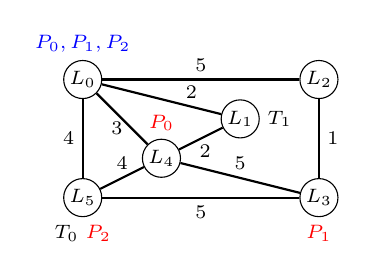
\begin{tikzpicture}[scale=0.5]
	\scriptsize
  \node[draw, circle, inner sep=1pt, label=above:{\textcolor{blue}{$P_0, P_1,P_2$}}] (l0) at (0,0) {$L_0$};
  \node[draw, circle, inner sep=1pt, label=right:{$T_1$}] (l1) at (4,-1) {$L_1$};
  \node[draw, circle, inner sep=1pt] (l2) at (6,0) {$L_2$};
  \node[draw, circle, inner sep=1pt, label=below:{\textcolor{red}{$P_1$}}] (l3) at (6,-3) {$L_3$};
  \node[draw, circle, inner sep=1pt, label=above:{\textcolor{red}{$P_0$}}] (l4) at (2,-2) {$L_4$};
  \node[draw, circle, inner sep=1pt, label=below:{$T_0$ \textcolor{red}{$P_2$}}] (l5) at (0,-3) {$L_5$};

  \draw[thick] (l0) to node[above] {5} (l2);
  \draw[thick] (l0) to node[above, pos=0.75] {2} (l1);
  \draw[thick] (l0) to node[below, pos=0.4] {3} (l4);
  \draw[thick] (l0) to node[left] {4} (l5);
  \draw[thick] (l2) to node[right] {1} (l3);
  \draw[thick] (l4) to node[below, pos=0.6] {2} (l1);
  \draw[thick] (l4) to node[above] {5} (l3);
  \draw[thick] (l5) to node[below] {5} (l3);
  \draw[thick] (l4) to node[above] {4} (l5);
\end{tikzpicture}
\vspace{-0.2cm}
\hspace{-0.6cm} \caption{Illustrative IPC NoMystery example.}
\label{fig:nomystery-example}
\vspace{-0.2cm}
\end{wrapfigure}

We define three kinds of action-set properties for this domain:
\emph{uses $T_i$ $(L_x,L_y)$} (truck $T_i$ drives at least once from
$L_x$ to $L_y$ or vice versa); \emph{doesn't use $T_i$ $(L_x,L_y)$}
(truck $T_i$ does not drive from $L_x$ to $L_y$ or vice versa);
\emph{same truck $P_x$ $P_y$} (both packages are delivered by the same
truck). We consider six instances of these properties: 1.\ uses $T_0$
$(L_2,L_3)$; 2.\ same truck $P_1$ $P_2$; 3.\ uses $T_0$ $(L_4,L_3)$;
4.\ same truck $P_2$ $P_0$; 5.\ doesn't use $T_0$ $(L_0,L_5)$;
6.\ uses $T_1$ $(L_5,L_4)$.

Fixing the package destinations as hard goals (defining the set of
plans \plans\ considered), and computing the MUGS over these six
action-set properties using the algorithms previously described, it
turns out there are 7 minimal unsolvable subsets of these properties,
each of size 3.

Say now that the current plan uses $T_0$ only, and includes the action
(drive T0 L5 L0). The user might ask \emph{''Why don't you avoid the
  road $L_0-L_5$, which has a lot of traffic at the
  moment?''}. Answering this question in terms of contrastive
explanation, as previously discussed, corresponds to forcing property
5 to be satisfied. At the same time, the plan already satisfies
properties 2 and 4. However, one of the MUGS is $\{2,4,5\}$, and hence
the answer to the user question would be: \textit{Because if you don't
  use that road, then you would not be able to deliver all packages
  using a single truck}.
